\chapter{Simulation d'inflorescences attractives} 
\label{chap:deb}

On détaille dans cette annexe comment simuler des dynamiques d'inflorescences attractives.
Pour ce faire, nous avons besoin des dates de débourrements des inflorescences ainsi que de la loi de mortalité des inflorescences.


Le \emph{dataset 1} contient des dates de débourrements. On ne pourra cependant pas les utiliser.
Dans le verger n\textdegree1, les dynamiques pour les modalités «enherbement ras» et «paillage synthétique» issues des deux jeux de données ont des dynamiques plutôt similaires ; on pourrait donc utiliser les débourrements du \emph{dataset 1} mis à l'échelle.
En revanche, pour la modalité «enherbement haut», on observe des dynamiques très différentes. 
Et comme l'on souhaite privilégier les dynamiques issues du \emph{dataset 2} (qui sont associées aux dynamiques de larves), il faut procéder autrement.
(Il en va de même pour les modalités «enherbement ras» et «paillage synthétique» du verger n\textdegree2.)
 
L'objectif est alors de simuler les dates de débourrements qui permettent de produire la dynamique d'inflorescences vivantes du \emph{dataset 2}.
Pour cela, on suppose que la durée de vie effective d'une inflorescence suit une loi normale.
On possède les durées de vies effectives dans le \emph{dataset 1}.
Premièrement, en fixant le risque de première espèce à $\alpha = 5\%$, un test de normalité de Shapiro--Wilk nous confirme la normalité ($p$-valeur de 0.05447, on ne rejette donc pas l'hypothèse de normalité).
Deuxièmement, on observe une durée de vie effective moyenne de 29 jours (avec un écart-type de 14).
Ainsi, il faut donc simuler des débourrements, pour que des inflorescences ayant une durée de vie qui suit une $\mathcal{N}\left( 29; 14 \right)$, donne la dynamique d'inflorescences vivantes du \emph{dataset 2}.
Il faut donc trouver les $B_t$ tels que 
\[
I_{t}^{2} = B_t + \sum_{j = 1}^{50} B_{t - j} \times \left( 1 - F\left( j \right) \right),  \qquad \text{ avec } B_{t} = 0 \text{ si } t \leq 0,
\]
où $F$ est la fonction de répartition d'une $\mathcal{N}\left( 29;14 \right)$ et 50 la durée de vie théorique d'une inflorescence.
 
Par souci d'homogénéité, on utilisera les débourrements simulés pour les trois modalités, et ce pour les deux vergers.



Les inflorescences \emph{attractives} peuvent alors se calculer en utilisant la formule
\[
I_{t}^{a} = B_t + \sum_{t = 1}^{d_A} B_{t-j} \times \left( 1 - F(j) \right), \qquad \text{ avec } B_{t} = 0 \text{ si } t \leq 0. 
\]
Ici, $B_t$ représente le nombre de débourrements à la date $t$, $d_A$ la durée d'attractivité voulue et $F$ la fonction de répartition d'une $\mathcal{N}\left( 29; 14 \right)$.

Dans notre cas, on choisira $d_A = 16$ jours, correspondant à la durée des stades C, D et E.

La figure~\ref{fig:compsimuobs} illustre la différence entre les inflorescences vivantes observées et les inflorescences vivantes simulées en utilisant la méthode décrite ci-dessus.

\begin{figure}[h]
\centering
 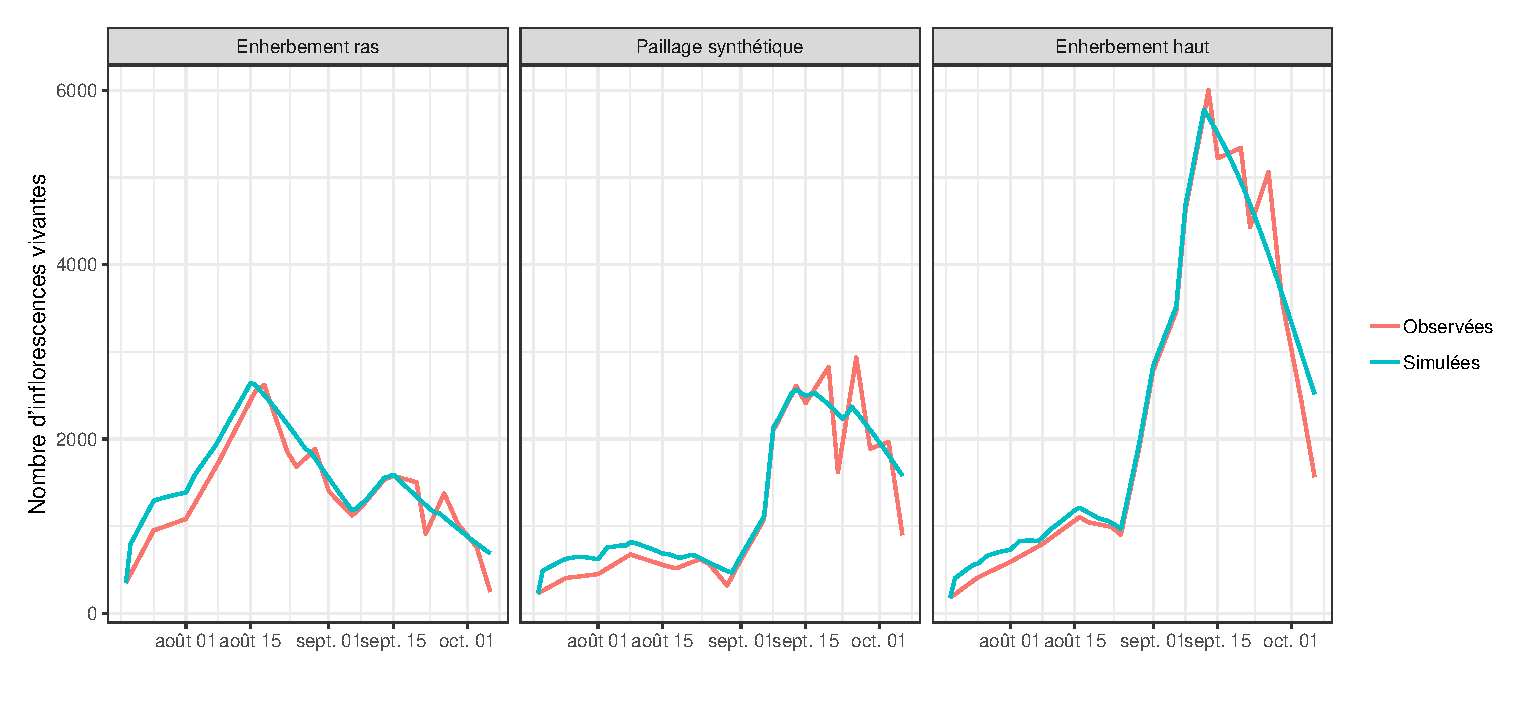
\epsfig{file = plots/simu_vs_obs.eps, scale = 0.59}
 \caption{Différences entre les inflorescences vivantes observées et simulées (verger n\textdegree1).}
 \label{fig:compsimuobs}
\end{figure}
